\documentclass[12pt]{article}
\usepackage{amsmath}
\usepackage{graphicx}
\usepackage{hyperref}
\usepackage{listings}
\usepackage{color}
\usepackage{pythonhighlight}
\usepackage{microtype} % Paket untuk meningkatkan penataan teks
\usepackage{xcolor}

\lstset{
    language=Python,
    backgroundcolor=\color{lightgray},   % Warna latar belakang
    basicstyle=\ttfamily\footnotesize,    % Ukuran dan font
    breaklines=true,                      % Memecah baris panjang
    keywordstyle=\color{blue},            % Warna untuk keyword
    stringstyle=\color{red},              % Warna untuk string
    commentstyle=\color{green},           % Warna untuk komentar
}

\title{Operating System Course Report - First Half of the Semester}
\author{A class}
\date{\today}

\begin{document}

\maketitle
\newpage

\tableofcontents
\newpage

\section{Introduction}
This report summarizes the topics covered during the first half of the Operating System course. It includes theoretical concepts, practical implementations, and assignments. The course focuses on the fundamentals of operating systems, including system architecture, process management, CPU scheduling, and deadlock handling.

\section{Course Overview}
\subsection{Objectives}
The main objectives of this course are:
\begin{itemize}
    \item To understand the basic components and architecture of a computer system.
    \item To learn process management, scheduling, and inter-process communication.
    \item To explore file systems, input/output management, and virtualization.
    \item To study the prevention and handling of deadlocks in operating systems.
\end{itemize}

\subsection{Course Structure}
The course is divided into two halves. This report focuses on the first half, which covers:
\begin{itemize}
    \item Basic Concepts and Components of Computer Systems
    \item System Performance and Metrics
    \item System Architecture of Computer Systems
    \item Process Description and Control
    \item Scheduling Algorithms
    \item Process Creation and Termination
    \item Introduction to Threads
    \item File Systems
    \item Input and Output Management
    \item Deadlock Introduction and Prevention
    \item User Interface Management
    \item Virtualization in Operating Systems
\end{itemize}

\section{Topics Covered}

\subsection{Basic Concepts and Components of Computer Systems}
This section explains the fundamental components that make up a computer system, including the CPU, memory, storage, and input/output devices.

\subsection{System Performance and Metrics}
This section introduces various system performance metrics used to measure the efficiency of a computer system, including throughput, response time, and utilization.

\subsection{System Architecture of Computer Systems}
Describes the architecture of modern computer systems, focusing on the interaction between hardware and the operating system.

\subsection{Process Description and Control}
Processes are a central concept in operating systems. This section covers:
\begin{itemize}
    \item Process states and state transitions
    \item Process control block (PCB)
    \item Context switching
\end{itemize}


\subsection{Scheduling Algorithms}
\subsubsection{Shortest Job Next (SJN)}

\begin{figure}[h]
    \centering
    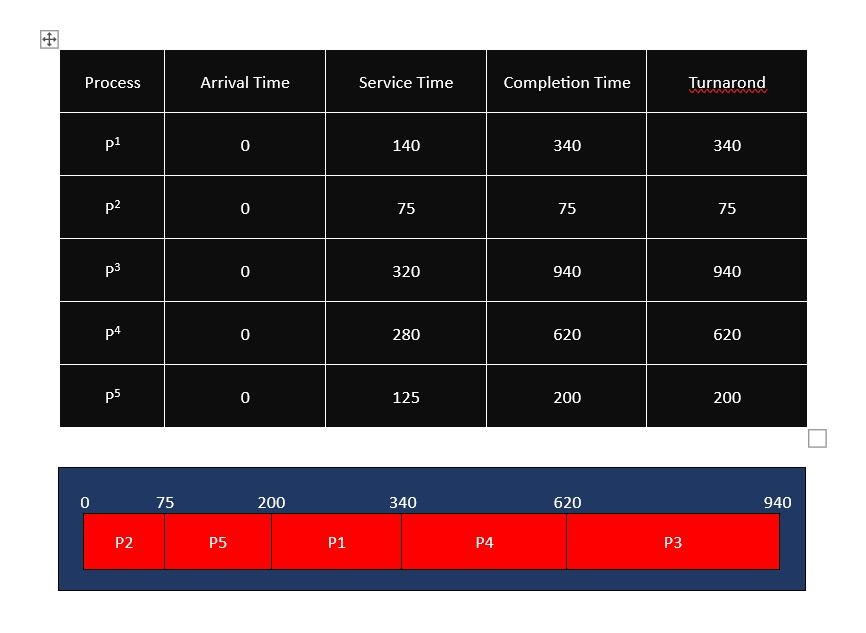
\includegraphics[width=1\textwidth]{asset/sjn-illustration.jpg}
    \caption{Ilustrasi SJN}
    \label{fig:ilustrasi sjn}
\end{figure}

 Dalam Shortest Job Next (SJN), saat memilih pekerjaan berikutnya untuk dijalankan, lihat semua proses dalam status siap dan jalankan yang memiliki waktu layanan tersingkat. Dalam kasus ini, kita perlu mengetahui waktu layanan pada setiap titik waktu tertentu. Ini adalah algoritma non -preemptif.Pekerjaan baru tidak akan diberi kesempatan pada CPU hingga pekerjaan saat ini selesai meskipun pekerjaan baru tersebut lebih pendek.
 \subsubsection{Konsep dan Istilah Utama}
\begin{itemize}
    \item Waktu layanan adalah jumlah waktu yang dibutuhkan suatu proses atau pekerjaan untuk menyelesaikan eksekusi setelah mulai berjalan pada CPU. Waktu layanan juga dikenal sebagai burst time.
    \item Waktu kedatangan adalah waktu saat suatu proses tiba dan siap untuk dieksekusi di CPU atau antrean penjadwalan.
    \item Waktu penyelesaian adalah titik waktu ketika suatu proses menyelesaikan eksekusinya.
    \item Waktu penyelesaian adalah total waktu yang dibutuhkan oleh suatu proses untuk menyelesaikan eksekusinya, sejak proses tersebut tiba di antrian siap hingga proses tersebut menyelesaikan eksekusi. Waktu penyelesaian dihitung sebagai waktu penyelesaian dikurangi waktu kedatangan.
    \item Algoritma penjadwalan nonpreemptif adalah algoritma yang mana proses yang telah mulai dijalankan akan terus berlanjut hingga proses tersebut selesai. Proses baru tidak diperbolehkan mengganggu proses yang sedang berjalan.
\end{itemize}

\subsubsection{Contoh Kasus Shortest Job Next (SJN) Scheduling}
    \begin{itemize}
        \item Pada server, terdapat beberapa proses yang membutuhkan CPU untuk waktu yang berbeda-beda. Misalnya, proses A membutuhkan 5 detik CPU, proses B membutuhkan 3 detik, dan proses C membutuhkan 1 detik.
        \item SJN memilih proses dengan waktu eksekusi tersingkat terlebih dahulu.Dalam kasus ini, sistem akan menjalankan proses C terlebih dahulu,kemudian B, dan terakhir A. Ini mengurangi waktu tunggu rata-rata karena proses yang lebih singkat diselesaikan lebih cepat.
    \end{itemize} 


 
    
\subsection{Process Creation and Termination}

\subsubsection{\textit{Process Creation}}
\begin{itemize}
    \item Definsi dan Konsep Dasar \textit{Process Creation}
    
    \begin{figure}[h]
        \centering
        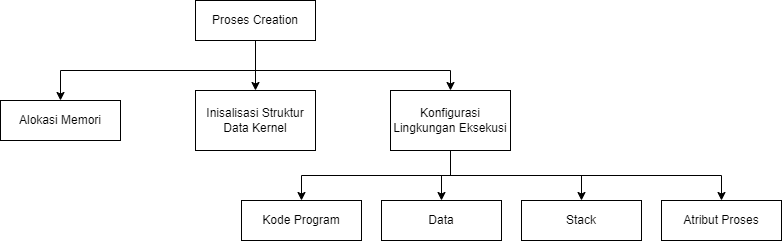
\includegraphics[width=1\textwidth]{D:/Universitas Hasanuddin/Semester III/Sistem Operasi/Repository/os_report_mid2024/a_class/asset/process-diagram.drawio.png}
        \caption{Diagram \textit{Process Creation} dan Komponen Proses}
    \end{figure}
    
    \textit{Process Creation}, atau penciptaan proses, adalah 
    salah satu fungsi fundamental dalam sistem operasi 
    modern. Ini merupakan mekanisme yang memungkinkan sistem 
    operasi untuk membuat unit eksekusi baru, yang kita kenal 
    sebagai proses, sehingga program dapat dijalankan di CPU. 
    Dalam konteks sistem operasi, proses didefinisikan sebagai 
    program yang sedang dieksekusi, yang terdiri atas kode 
    program, data, \textit{stack}, dan berbagai atribut 
    yang dikelola oleh sistem operasi (Tanenbaum \& Bos, 2015).

    Ketika sebuah proses baru dibuat, sistem operasi harus 
    melakukan serangkaian operasi kompleks untuk memastikan 
    bahwa proses tersebut memiliki semua sumber daya yang 
    diperlukan untuk eksekusi yang benar. Ini termasuk alokasi 
    ruang memori, inisialisasi struktur data \textit{kernel}, dan 
    konfigurasi lingkungan eksekusi. Proses penciptaan ini 
    sangat penting karena menjadi fondasi bagi \textit{multitasking} 
    dan manajemen sumber daya dalam sistem operasi modern.

    \item Alasan Dibuatnya Proses
    
    Ada beberapa alasan mengapa sistem operasi perlu membuat 
    proses baru. Pertama, dan yang paling umum, adalah untuk 
    menjalankan program baru. Ketika pengguna atau sistem 
    meminta eksekusi sebuah program, sistem operasi harus 
    membuat proses baru untuk mengakomodasi program tersebut. 
    Ini melibatkan pembacaan file \textit{executable}, alokasi 
    memori, dan persiapan lingkungan eksekusi 
    (Silberschatz et al., 2018).

    Kedua, proses \textit{creation} mendukung konsep 
    \textit{multiprogramming}. \textit{Multiprogramming} 
    memungkinkan beberapa program berjalan secara bersamaan 
    (atau lebih tepatnya, bergantian dengan sangat cepat) pada 
    sistem dengan satu atau lebih \textit{core}. Ini meningkatkan 
    efisiensi penggunaan \textit{core} dan responsivitas sistem 
    secara keseluruhan. Sistem operasi membuat dan mengelola 
    beberapa proses, serta beralih di antara mereka dengan cepat 
    untuk memberikan ilusi bahwa mereka berjalan secara bersamaan 
    pada \textit{core} yang ada.

    \begin{figure}[h]
        \centering
        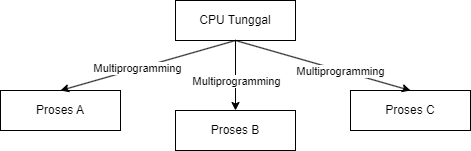
\includegraphics[width=1\textwidth]{D:/Universitas Hasanuddin/Semester III/Sistem Operasi/Repository/os_report_mid2024/a_class/asset/multiprogramming-diagram.drawio.png}
        \caption{Diagram Ilustrasi \textit{Multiprogramming}}
    \end{figure}

    Ketiga, proses \textit{creation} memfasilitasi pemrosesan 
    paralel pada sistem dengan beberapa \textit{core}. Dalam 
    skenario ini, sistem operasi dapat membuat beberapa proses 
    yang benar-benar berjalan secara bersamaan pada \textit{core} 
    yang berbeda. Setiap \textit{core} dapat menangani tugas 
    secara independen, sehingga meningkatkan \textit{throughput} sistem 
    secara signifikan dan memungkinkan eksekusi beberapa tugas 
    secara simultan.

    \begin{figure}[h]
        \centering
        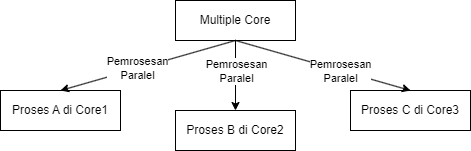
\includegraphics[width=1\textwidth]{D:/Universitas Hasanuddin/Semester III/Sistem Operasi/Repository/os_report_mid2024/a_class/asset/pemrosesan-paralel-illustration.drawio.png}
        \caption{Diagram Ilustrasi Pemerosesan Paralel}
    \end{figure}

    \item Elemen Penting Dalam \textit{Process Creation}
    
    \begin{itemize}
        \item ID Proses
        
        Setiap proses yang dibuat oleh sistem operasi diberi 
        sebuah pengenal unik yang disebut \textit{Process ID} 
        atau PID. PID ini sangat penting untuk manajemen proses 
        oleh sistem operasi. Menurut Love (2010), di sistem 
        Linux, PID diimplementasikan sebagai bilangan bulat yang 
        diincrement setiap kali proses baru dibuat. Ketika nilai 
        PID mencapai nilai maksimum (biasanya 32.768 pada banyak 
        sistem), sistem akan melakukan \textit{wrap-around} dan 
        mulai lagi dari nilai terendah yang tersedia.

        Implementasi PID melibatkan struktur data yang efisien 
        untuk alokasi dan dealokasi yang cepat. Misalnya, sistem 
        Linux menggunakan bitmap untuk melacak PID yang tersedia. 
        Ini memungkinkan alokasi PID baru dalam waktu konstan, 
        yang sangat penting mengingat frekuensi tinggi operasi 
        pembuatan proses dalam sistem modern.

        \begin{figure}[h]
            \centering
            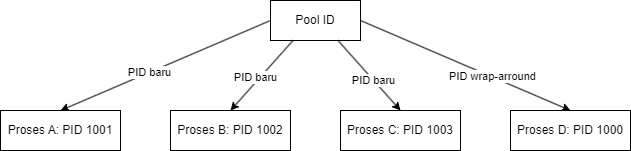
\includegraphics[width=1\textwidth]{D:/Universitas Hasanuddin/Semester III/Sistem Operasi/Repository/os_report_mid2024/a_class/asset/pid-illustration.drawio.png}
            \caption{Diagram Alokasi PID}
        \end{figure}

        \item Pewarisan
        
        Konsep pewarisan dalam konteks \textit{process creation} 
        mengacu pada transfer atribut dan sumber daya dari proses 
        induk ke proses anak. Ini adalah aspek kunci dari model 
        proses UNIX dan turunannya. Ketika sebuah proses anak 
        dibuat (misalnya melalui pemanggilan sistem 
        \textit{fork()} di UNIX), ia mewarisi banyak atribut dari 
        induknya.

        Atribut yang diwariskan biasanya meliputi prioritas 
        penjadwalan, grup proses, direktori kerja, dan variabel 
        lingkungan. Selain itu, proses anak juga mewarisi salinan 
        dari tabel \textit{file descriptor} induk, yang berarti 
        ia memiliki akses ke file yang sama yang terbuka oleh 
        induknya saat \textit{fork()} terjadi (Bovet \& Cesati, 
        2005).

        Namun, penting untuk dicatat bahwa pewarisan ini tidak 
        selalu berarti penyalinan langsung. Banyak sistem operasi 
        modern menggunakan teknik \textit{copy-on-write} untuk 
        efisiensi. Dalam skema ini, proses anak awalnya berbagi 
        halaman memori fisik yang sama dengan induknya. Hanya 
        ketika salah satu proses mencoba memodifikasi sebuah 
        halaman, salinan terpisah dibuat. Ini secara signifikan 
        mengurangi \textit{overhead} pembuatan proses.

        \item Alokasi Sumber daya
        
        Alokasi sumber daya adalah aspek kritis dari 
        \textit{process creation}. Ketika sebuah proses baru 
        dibuat, sistem operasi harus mengalokasikan berbagai 
        sumber daya yang dibutuhkan proses untuk berfungsi. Ini 
        meliputi memori, \textit{file descriptor}, dan waktu CPU.

        Alokasi memori melibatkan penciptaan ruang alamat virtual 
        untuk proses baru. Pada sistem modern, ini biasanya 
        melibatkan pengaturan struktur \textit{page table} yang 
        memetakan alamat virtual ke alamat fisik. Sistem operasi 
        juga harus mengalokasikan memori untuk \textit{stack} 
        proses, yang digunakan untuk menyimpan variabel lokal dan 
        informasi pemanggilan fungsi.

        Menurut Arpaci-Dusseau (2018), alokasi 
        sumber daya juga melibatkan inisialisasi berbagai struktur 
        data \textit{kernel} yang terkait dengan proses. Ini 
        termasuk \textit{Process Control Block} (PCB) atau 
        \textit{task\_struct} di Linux, yang menyimpan semua 
        informasi yang dibutuhkan \textit{kernel} untuk mengelola 
        proses.

        \item Hubungan Induk-anak
        
        Sistem operasi memelihara hubungan hierarkis antara 
        proses, yang dikenal sebagai hubungan induk-anak. Ketika 
        sebuah proses membuat proses baru, proses asli disebut 
        induk, dan proses baru disebut anak. Hubungan ini penting 
        untuk berbagai aspek manajemen proses, termasuk terminasi 
        proses dan propagasi sinyal.

        Di sistem berbasis UNIX, hubungan induk-anak 
        diimplementasikan melalui \textit{pointer} dalam struktur 
        proses. Setiap proses memiliki \textit{pointer} ke proses 
        induknya, serta daftar proses anaknya. Ini memungkinkan 
        penjelajahan yang efisien dari pohon proses, yang diperlukan 
        untuk operasi seperti terminasi proses dan pembersihan 
        sumber daya (Bovet \& Cesati, 2005).

        Hubungan induk-anak juga memainkan peran penting dalam 
        penanganan sinyal dan pengumpulan status terminasi. 
        Ketika sebuah proses berakhir, sistem operasi mengirim 
        sinyal \textit{SIGCHLD} ke proses induk, memungkinkannya 
        untuk melakukan tindakan yang sesuai, seperti 
        mengumpulkan status keluar dari proses anak atau 
        membersihkan sumber daya.

    \end{itemize}

    \item Tahapan \textit{Process Creation}
    
    \textit{Proses creation} adalah operasi kompleks yang melibatkan beberapa tahap. Meskipun implementasi spesifik dapat bervariasi antar sistem operasi, tahapan umumnya adalah sebagai berikut:
    \begin{itemize}
        \item Permintaan Proses
        
        Proses \textit{creation} biasanya dimulai dengan 
        permintaan eksplisit, baik dari pengguna (misalnya, 
        menjalankan program dari \textit{command line}) atau dari 
        proses yang sudah berjalan (misalnya, server web yang 
        membuat proses baru untuk menangani koneksi masuk). 
        Dalam sistem berbasis UNIX, ini sering dipicu oleh 
        pemanggilan sistem \textit{fork()} atau salah satu 
        variannya.

        Ketika \textit{fork()} dipanggil, sistem operasi 
        pertama-tama memeriksa apakah ada sumber daya sistem 
        yang cukup untuk mendukung proses baru. Ini termasuk 
        pemeriksaan batas jumlah proses sistem dan batas 
        per-pengguna. Jika sumber daya tidak mencukupi, 
        pemanggilan sistem akan gagal dengan kode kesalahan yang 
        sesuai (Love, 2010).

        \item Penugasan PID 
        
        Jika sumber daya mencukupi, langkah berikutnya adalah 
        mengalokasikan PID untuk proses baru. Seperti disebutkan 
        sebelumnya, ini biasanya melibatkan pemilihan bilangan 
        bulat berikutnya yang tersedia dari \textit{pool} PID. 
        Sistem operasi harus memastikan bahwa PID yang dipilih 
        unik dan belum digunakan oleh proses lain yang sedang 
        berjalan.

        Di Linux, alokasi PID diimplementasikan dengan cara yang 
        aman untuk \textit{thread} (\textit{thread-safe}) guna 
        menghindari \textit{race condition} di sistem 
        multiprosesor. Ini melibatkan penggunaan struktur data 
        \textit{atomic} dan mekanisme \textit{locking} untuk 
        memastikan bahwa dua proses tidak pernah mendapatkan PID 
        yang sama (Love, 2010).

        \item Alokasi Sumber Daya 
        
        Setelah PID dialokasikan, sistem operasi mulai 
        mengalokasikan sumber daya yang diperlukan untuk proses 
        baru. Ini adalah tahap yang kompleks dan melibatkan 
        beberapa sub-langkah:

        \begin{enumerate}
            \item Alokasi struktur \textit{kernel}: Sistem mengalokasikan dan menginisialisasi \textit{Process Control Block} (PCB) atau ekuivalennya. PCB menyimpan semua informasi yang diperlukan sistem untuk mengelola proses, termasuk status proses, prioritas penjadwalan, dan \textit{pointer} ke struktur data terkait lainnya.
            \item Alokasi memori: Sistem membuat ruang alamat virtual untuk proses baru. Pada sistem modern, ini biasanya melibatkan pengaturan struktur \textit{page table}. Jika proses baru adalah hasil dari \textit{fork()}, sistem mungkin menggunakan teknik \textit{copy-on-write} untuk efisiensi.
            \item Inisialisasi \textit{stack}: Sistem mengalokasikan dan menginisialisasi \textit{stack} untuk proses baru. \textit{Stack} digunakan untuk menyimpan variabel lokal, parameter fungsi, dan alamat kembali (\textit{return address}).
            \item Duplikasi deskriptor file: Jika proses baru adalah hasil dari \textit{fork()}, sistem menduplikasi tabel \textit{file descriptor} dari proses induk.
            \item Inisialisasi penjadwalan: Sistem menginisialisasi struktur data penjadwalan untuk proses baru, termasuk pengaturan prioritas awal dan statistik penggunaan CPU.
        \end{enumerate}

        \item Pembuatan PCB
        
        \textit{Process Control Block} (PCB) adalah struktur data inti 
        yang digunakan sistem operasi untuk melacak status dan 
        sumber daya proses. Pembuatan PCB melibatkan inisialisasi 
        berbagai \textit{field} dengan nilai yang sesuai.

        Pembuatan PCB adalah langkah kritis dalam proses \textit{creation} 
        karena struktur ini menjadi referensi utama sistem operasi untuk 
        semua operasi yang melibatkan proses tersebut di masa mendatang.
    \end{itemize}
    
    
\end{itemize}


Setelah semua tahapan ini selesai, proses baru siap untuk 
dijadwalkan dan dieksekusi. Pada titik ini, sistem operasi dapat 
memilih untuk segera menjadwalkan proses baru untuk eksekusi, 
atau menempatkannya dalam antrian proses yang siap, tergantung 
pada kebijakan penjadwalan dan beban sistem saat itu.

\subsubsection{Siapa yang Membuat Proses}
(Isi materi disini)

\subsubsection{Proses \textit{Termination}}
\begin{itemize}
    \item Definisi Proses \textit{Termination}
    
    (isi materi disini)

    \item Jenis-jenis \textit{Termination}
    
    (Isi materi disini)

    \item Apa yang Terjadi Setelah \textit{Termination}
    
    (isi materi disini)
\end{itemize}

\begin{thebibliography}{99}

    \bibitem{arpaci2018} 
    Arpaci-Dusseau, R. H., \& Arpaci-Dusseau, A. C. (2018). \textit{Operating Systems: Three Easy Pieces}. Arpaci-Dusseau Books.

    \bibitem{bovet2005} 
    Bovet, D. P., \& Cesati, M. (2005). \textit{Understanding the Linux Kernel} (3rd ed.). O'Reilly Media.

    \bibitem{love2010} 
    Love, R. (2010). \textit{Linux Kernel Development} (3rd ed.). Addison-Wesley Professional.

    \bibitem{silberschatz2018} 
    Silberschatz, A., Galvin, P. B., \& Gagne, G. (2018). \textit{Operating System Concepts} (10th ed.). John Wiley \& Sons.

    \bibitem{tanenbaum2015} 
    Tanenbaum, A. S., \& Bos, H. (2015). \textit{Modern Operating Systems} (4th ed.). Pearson.

\end{thebibliography}

\subsection{Introduction to Threads}
This section introduces the concept of threads and their relation to processes, covering:
\begin{itemize}
    \item Single-threaded vs. multi-threaded processes
    \item Benefits of multithreading
\end{itemize}

\begin{figure}[h]
    \centering
    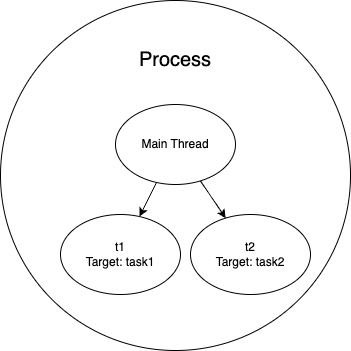
\includegraphics[width=0.5\textwidth]{D:/Universitas Hasanuddin/Semester III/Sistem Operasi/Repository/os_report_mid2024/a_class/asset/example.png}  % Sesuaikan nama file dan ukurannya
    \caption{Ini adalah gambar contoh dari multithreading.}
    \label{fig:contoh_gambar}
\end{figure}

Seperti yang terlihat pada Gambar \ref{fig:contoh_gambar}, inilah cara menambahkan gambar dengan keterangan.

\subsection{File Systems}
File systems provide a way for the operating system to store, retrieve, and manage data. This section explains:
\begin{itemize}
    \item File system structure
    \item File access methods
    \item Directory management
\end{itemize}

\subsection{Input and Output Management}
Input and output management is key for handling the interaction between the system and external devices. This section includes:
\begin{itemize}
    \item Device drivers
    \item I/O scheduling
\end{itemize}

\subsection{Deadlock Introduction and Prevention}
Explores the concept of deadlocks and methods for preventing them:
\begin{itemize}
    \item Deadlock conditions
    \item Deadlock prevention techniques
\end{itemize}

\subsection{User Interface Management}
This section discusses the role of the operating system in managing the user interface. Topics covered include:
\begin{itemize}
    \item Graphical User Interface (GUI)
    \item Command-Line Interface (CLI)
    \item Interaction between the user and the operating system
\end{itemize}

\subsection{Virtualization in Operating Systems}
Virtualization allows multiple operating systems to run concurrently on a single physical machine. This section explores:
\begin{itemize}
    \item Concept of virtualization
    \item Hypervisors and their types
    \item Benefits of virtualization in modern computing
\end{itemize}

\section{Assignments and Practical Work}
\subsection{Assignment 1: Process Scheduling}
Students were tasked with implementing various process scheduling algorithms (e.g., FCFS, SJN, and RR) and comparing their performance under different conditions.
\subsubsection{Group 1}
\begin{python}
    class Process:
    def __init__(self, pid, arrival_time, burst_time):
        self.pid = pid
        self.arrival_time = arrival_time
        self.burst_time = burst_time
        self.completion_time = 0
        self.turnaround_time = 0
        self.waiting_time = 0
\end{python}

\begin{table}[htbp] % Optional: For floating position
    \centering
    \begin{tabular}{|c|c|c|} % Defines number of columns and alignment (c = center, l = left, r = right). '|' creates vertical lines.
    \hline
    Header 1 & Header 2 & Header 3 \\ % Column headers
    \hline
    Row 1, Column 1 & Row 1, Column 2 & Row 1, Column 3 \\ % First row of data
    \hline
    Row 2, Column 1 & Row 2, Column 2 & Row 2, Column 3 \\ % Second row of data
    \hline
    \end{tabular}
    \caption{Your table caption} % Optional: For adding a caption
    \label{tab:your_label} % Optional: For cross-referencing the table
\end{table}

\subsubsection{Group 6}
\textbf{Soal:}

Implementasikan algoritma penjadwalan proses FCFS (\textit{First Come First Serve}), SJN (\textit{Shortest Job Next}), dan RR (\textit{Round Robin}) menggunakan Python. Bandingkan kinerja ketiga algoritma tersebut dengan menggunakan set data berikut:
    \begin{table}[h] % Optional: For floating position
        \centering
        \begin{tabular}{|c|c|c|} % Defines number of columns and alignment (c = center, l = left, r = right). '|' creates vertical lines.
        \hline
        Proses & Waktu Kedatangan & Waktu Burst \\ % Column headers
        \hline
        P1 & 0 & 10 \\ % First row of data
        \hline
        P2 & 1 & 4 \\ % Second row of data
        \hline
        P3 & 3 & 2 \\
        \hline
        P4 & 5 & 1 \\
        \hline
        \end{tabular}
        \caption{Data Proses Untuk Penjadwalan} % Optional: For adding a caption
        \label{tab:Data Proses Untuk Penjadwalan} % Optional: For cross-referencing the table
    \end{table}

Untuk algoritma \textit{Round Robin}, gunakan kuantum waktu dua unit. Hitung waktu tunggu rata-rata dan waktu penyelesaian rata-rata untuk setiap algoritma.

\textbf{Jawaban:}
\begin{lstlisting}
class Process:
    def __init__(self, pid, arrival_time, burst_time):
        self.pid = pid
        self.arrival_time = arrival_time
        self.burst_time = burst_time
        self.remaining_time = burst_time
        self.completion_time = 0
        self.waiting_time = 0

    def fcfs(processes):
        time = 0
        for p in processes:
            if time < p.arrival_time:
                time = p.arrival_time
            p.waiting_time = time - p.arrival_time
            time += p.burst_time
            p.completion_time = time

    def sjn(processes):
        time = 0
        remaining = processes.copy()
        completed = []
        
        while remaining:
            available = [p for p in remaining if p.arrival_time <= time]
            if not available:
                time += 1
                continue
            
            next_process = min(available, key=lambda p: p.burst_time)
            next_process.waiting_time = time - next_process.arrival_time
            time += next_process.burst_time
            next_process.completion_time = time
            remaining.remove(next_process)
            completed.append(next_process)
        
        return completed

    def round_robin(processes, quantum):
        time = 0
        remaining = processes.copy()
        queue = []
        
        while remaining or queue:
            # Tambahkan proses yang baru tiba ke antrian
            new_arrivals = [p for p in remaining if p.arrival_time <= time and p not in queue]
            queue.extend(new_arrivals)
            for p in new_arrivals:
                remaining.remove(p)
            
            if not queue:
                time += 1
                continue
            
            current_process = queue.pop(0)
            if current_process.remaining_time <= quantum:
                time += current_process.remaining_time
                current_process.completion_time = time
                current_process.waiting_time += time - current_process.arrival_time - current_process.burst_time
            else:
                time += quantum
                current_process.remaining_time -= quantum
                current_process.waiting_time += time - current_process.arrival_time - (current_process.burst_time - current_process.remaining_time)
                
                # Tambahkan proses yang baru tiba selama eksekusi quantum
                new_arrivals = [p for p in remaining if p.arrival_time <= time and p not in queue]
                queue.extend(new_arrivals)
                for p in new_arrivals:
                    remaining.remove(p)
                
                queue.append(current_process)

    def calculate_averages(processes):
        avg_waiting_time = sum(p.waiting_time for p in processes) / len(processes)
        avg_turnaround_time = sum(p.completion_time - p.arrival_time for p in processes) / len(processes)
        return avg_waiting_time, avg_turnaround_time

# Data proses
processes = [
    Process("P1", 0, 10),
    Process("P2", 1, 4),
    Process("P3", 3, 2),
    Process("P4", 5, 1)
]

# FCFS
fcfs_processes = [Process(p.pid, p.arrival_time, p.burst_time) for p in processes]
fcfs(fcfs_processes)
fcfs_avg_waiting, fcfs_avg_turnaround = calculate_averages(fcfs_processes)

# SJN
sjn_processes = [Process(p.pid, p.arrival_time, p.burst_time) for p in processes]
sjn_completed = sjn(sjn_processes)
sjn_avg_waiting, sjn_avg_turnaround = calculate_averages(sjn_completed)

# Round Robin
rr_processes = [Process(p.pid, p.arrival_time, p.burst_time) for p in processes]
round_robin(rr_processes, 2)
rr_avg_waiting, rr_avg_turnaround = calculate_averages(rr_processes)
\end{lstlisting}

\textbf{\textit{Output:}}

\begin{figure}[h]
    \centering
    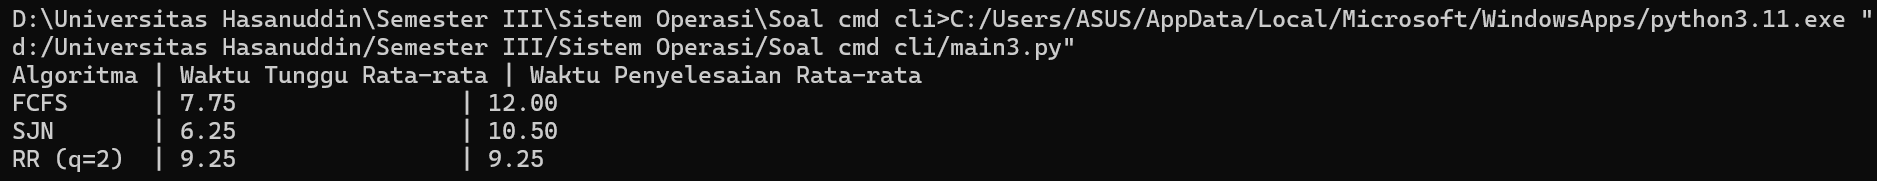
\includegraphics[width=1\textwidth]{D:/Universitas Hasanuddin/Semester III/Sistem Operasi/Repository/os_report_mid2024/a_class/asset/Screenshot 2024-10-03 120048.png}
    \caption{\textit{Ouput} Kode}
\end{figure}

\textbf{Kesimpulan:}

Dari hasil \textit{output} tersebut, kita bisa menyimpulkan bahwa:

\begin{itemize}
    \item Algoritma SJN memberikan waktu tunggu dan waktu penyelesaian yang paling rendah di antara ketiga algoritma tersebut.
    \item FCFS memiliki waktu tunggu dan waktu penyelesaian yang tertinggi.
    \item Algoritma \textit{Round Robin} dengan kuantum waktu dua unit menunjukkan waktu penyelesaian yang efisien, tetapi waktu tunggu rata-rata yang lebih tinggi dibandingkan SJN.
\end{itemize}

\subsection{Assignment 2: Deadlock Handling}

\subsubsection{Pertanyaan dan Jawaban serta Implementasi Kode Python untuk Deadlock Handling}

\textbf{Pertanyaan :} 

\vspace{0.2cm}

Jelaskan bagaimana deadlock dapat terjadi dalam kode di bawah!

\vspace{0.2cm}

\begin{python}
import threading
import time

class SumberDaya:
    def _init_(self, nama):
        self.nama = nama
        self.lock = threading.Lock()

def skenario_deadlock(sumber_a, sumber_b):
    def thread_1():
        # Kunci sumber daya dalam urutan yang sama di kedua thread
        with sumber_a.lock:
            print(f"Thread 1: Mengunci {sumber_a.nama}")
            time.sleep(1)  # Simulasikan kerja
            with sumber_b.lock:
                print(f"Thread 1: Mengunci {sumber_b.nama}")
        print("Thread 1 selesai")

    def thread_2():
        # Kunci sumber daya dalam urutan yang sama di kedua thread
        with sumber_a.lock:
            print(f"Thread 2: Mengunci {sumber_a.nama}")
            time.sleep(1)  # Simulasikan kerja
            with sumber_b.lock:
                print(f"Thread 2: Mengunci {sumber_b.nama}")
        print("Thread 2 selesai")

    t1 = threading.Thread(target=thread_1)
    t2 = threading.Thread(target=thread_2)

    t1.start()
    t2.start()
    
    t1.join()
    t2.join()

# Buat dua sumber daya
sumber_a = SumberDaya("Sumber Daya A")
sumber_b = SumberDaya("Sumber Daya B")
skenario_deadlock(sumber_a, sumber_b)
\end{python} 

\textbf{Jawaban:} Deadlock terjadi ketika dua thread mencoba mengunci dua sumber daya dalam urutan yang berlawanan. Dalam kode ini:

\begin{itemize}
    \item {thread\_1} mengunci {sumber\_a} terlebih dahulu, lalu mencoba mengunci {sumber\_b}.
    \item {thread\_2} mengunci {sumber\_b} terlebih dahulu, lalu mencoba mengunci {sumber\_a}. Jika {thread\_1} mengunci {sumber\_a} dan {thread\_2} mengunci {sumber\_b} pada saat yang sama, kedua thread akan menunggu selamanya untuk sumber daya lain yang tidak pernah tersedia, sehingga terjadi deadlock.
\end{itemize}




\subsection{Assignment 3: Multithreading and Amdahl's Law}
This assignment involved designing a multithreading scenario to solve a computationally intensive problem. Students then applied **Amdahl's Law** to calculate the theoretical speedup of the program as the number of threads increased.

\subsection{Assignment 4: Simple Command-Line Interface (CLI) for User Interface Management}
Students were tasked with creating a simple **CLI** for user interface management. The CLI should support basic commands such as file manipulation (creating, listing, and deleting files), process management, and system status reporting.

\subsection{Assignment 5: File System Access}
\subsubsection{Group 6}
\textbf{Soal:}

Anda diminta untuk melakukan tugas-tugas berikut:

\begin{enumerate}
    \item Membuat direktori baru bernama \texttt{ProyekA}.
    \item Di dalam direktori \texttt{ProyekA}, buat tiga berkas teks baru bernama \texttt{file1.txt}, \texttt{file2.txt}, dan \texttt{file3.txt}.
    \item Tuliskan "Hello World" ke dalam berkas \texttt{file1.txt}.
    \item Tampilkan isi dari \texttt{file1.txt} ke layar.
    \item Hapus berkas \texttt{file2.txt}.
    \item Ganti nama berkas \texttt{file3.txt} menjadi \texttt{file\_final.txt}.
\end{enumerate}

Tulis kode python untuk menyelesaikan tugas di atas.

\textbf{Jawaban:}

\begin{lstlisting}
import os

def main():
    # 1. Membuat direktori baru bernama ProyekA
    os.mkdir("ProyekA")
    print("Direktori ProyekA berhasil dibuat.")
    
    # Pindah ke direktori ProyekA
    os.chdir("ProyekA")
    print("Berpindah ke direktori ProyekA.")

    # 2. Membuat tiga berkas teks baru
    for file in ["file1.txt", "file2.txt", "file3.txt"]:
        with open(file, "w") as f:
            pass
    print("Berkas file1.txt, file2.txt, dan file3.txt berhasil dibuat.")
    
    # 3. Menuliskan "Hello World" ke dalam file1.txt
    with open("file1.txt", "w") as f:
        f.write("Hello World")
    print("Berhasil menulis 'Hello World' ke file1.txt.")
    
    # 4. Menampilkan isi dari file1.txt ke layar
    print("\nIsi dari file1.txt:")
    with open("file1.txt", "r") as f:
        print(f.read())
    
    # 5. Menghapus berkas file2.txt
    os.remove("file2.txt")
    print("\nBerkas file2.txt berhasil dihapus.")
    
    # 6. Mengganti nama berkas file3.txt menjadi file_final.txt
    os.rename("file3.txt", "file_final.txt")
    print("Berkas file3.txt berhasil diubah namanya menjadi file_final.txt.")
    
    # Menampilkan isi direktori akhir
    print("\nIsi direktori ProyekA setelah semua operasi:")
    print(os.listdir())
    
if __name__ == "__main__":
    main()
\end{lstlisting}

\newpage
\textbf{Output:}
\begin{figure}[h]
    \centering
    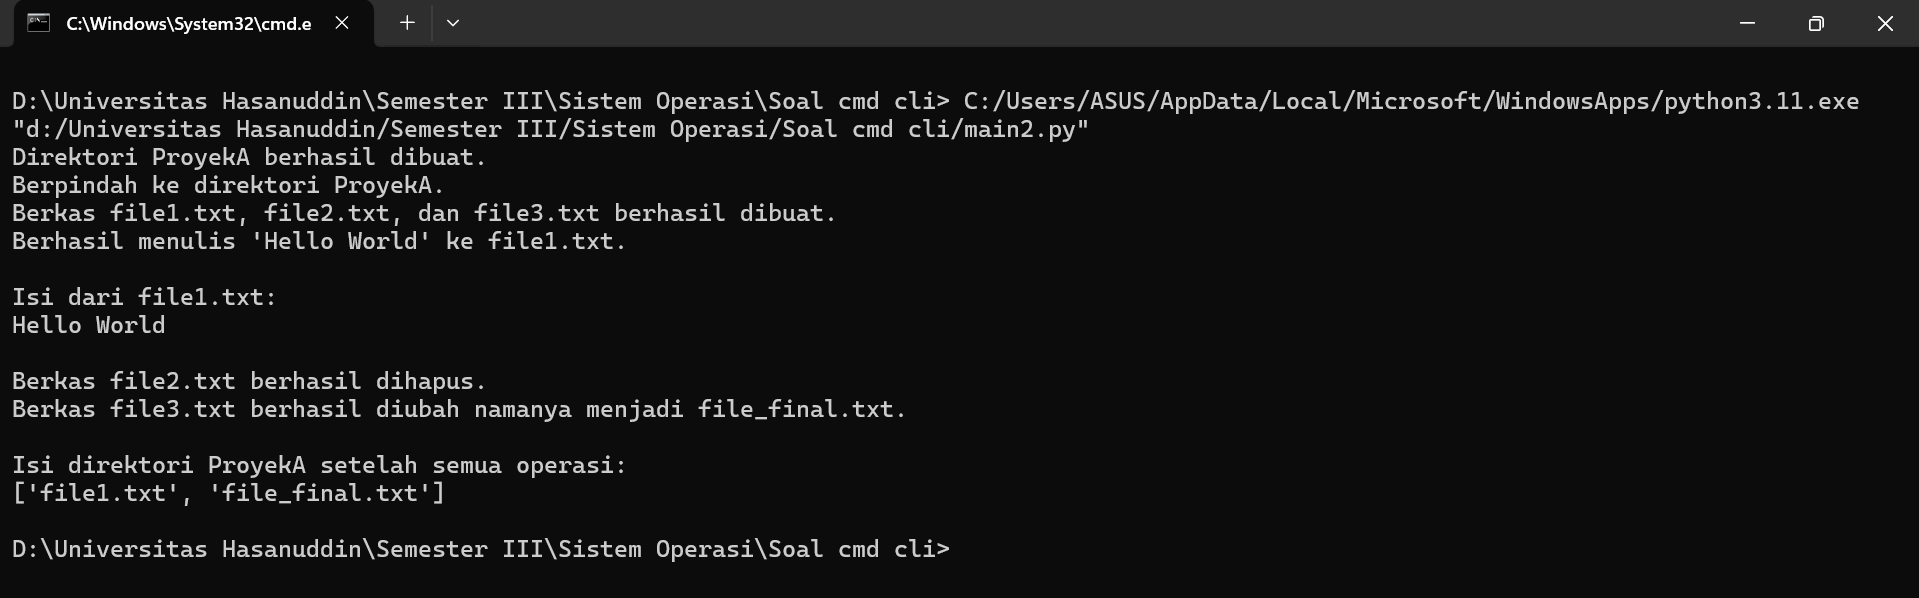
\includegraphics[width=1\textwidth]{D:/Universitas Hasanuddin/Semester III/Sistem Operasi/Repository/os_report_mid2024/a_class/asset/Screenshot 2024-10-03 115044.png}
    \caption{\textit{Ouput}}
    
\end{figure}

\section{Conclusion}
The first half of the course introduced core operating system concepts, including process management, scheduling, multithreading, and file system access. These topics provided a foundation for more advanced topics to be covered in the second half of the course.

\end{document}
